\subsection{UC7 - Riprendi trasferimento}
\begin{figure}[H]
    \centering
    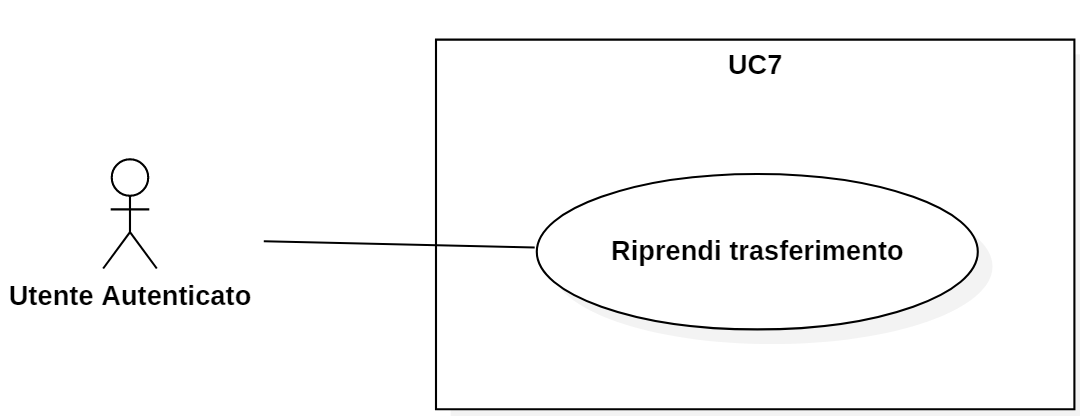
\includegraphics[scale = 0.4]{components/img/UC7.png}
    \caption{UC7 - Riprendi trasferimento}
\end{figure}
\begin{itemize}
\item \textbf{Attore Primario:} Utente autenticato;
\item \textbf{Precondizione:} L'utente ha a disposizione la possibilità di riprendere il trasferimento di un file messo precedentemente in pausa;
\item \textbf{Postcondizione:} Viene modificato lo stato del file da trasferimento in pausa a trasferimento in corso;
\item \textbf{Scenario principale:}
    \begin{enumerate}
    \item L'utente può riprendere il trasferimento di un file che si trova nello stato di trasferimento in pausa.
    \end{enumerate}
\end{itemize}